
%% bare_jrnl_transmag.tex
%% V1.4a
%% 2014/09/17
%% by Michael Shell
%% see http://www.michaelshell.org/
%% for current contact information.
%%
%% This is a skeleton file demonstrating the use of IEEEtran.cls
%% (requires IEEEtran.cls version 1.8a or later) with an IEEE 
%% Transactions on Magnetics journal paper.
%%
%% Support sites:
%% http://www.michaelshell.org/tex/ieeetran/
%% http://www.ctan.org/tex-archive/macros/latex/contrib/IEEEtran/
%% and
%% http://www.ieee.org/

%%*************************************************************************
%% Legal Notice:
%% This code is offered as-is without any warranty either expressed or
%% implied; without even the implied warranty of MERCHANTABILITY or
%% FITNESS FOR A PARTICULAR PURPOSE! 
%% User assumes all risk.
%% In no event shall IEEE or any contributor to this code be liable for
%% any damages or losses, including, but not limited to, incidental,
%% consequential, or any other damages, resulting from the use or misuse
%% of any information contained here.
%%
%% All comments are the opinions of their respective authors and are not
%% necessarily endorsed by the IEEE.
%%
%% This work is distributed under the LaTeX Project Public License (LPPL)
%% ( http://www.latex-project.org/ ) version 1.3, and may be freely used,
%% distributed and modified. A copy of the LPPL, version 1.3, is included
%% in the base LaTeX documentation of all distributions of LaTeX released
%% 2003/12/01 or later.
%% Retain all contribution notices and credits.
%% ** Modified files should be clearly indicated as such, including  **
%% ** renaming them and changing author support contact information. **
%%
%% File list of work: IEEEtran.cls, IEEEtran_HOWTO.pdf, bare_adv.tex,
%%                    bare_conf.tex, bare_jrnl.tex, bare_conf_compsoc.tex,
%%                    bare_jrnl_compsoc.tex, bare_jrnl_transmag.tex
%%*************************************************************************


% *** Authors should verify (and, if needed, correct) their LaTeX system  ***
% *** with the testflow diagnostic prior to trusting their LaTeX platform ***
% *** with production work. IEEE's font choices and paper sizes can       ***
% *** trigger bugs that do not appear when using other class files.       ***                          ***
% The testflow support page is at:
% http://www.michaelshell.org/tex/testflow/



\documentclass[journal]{IEEEtran}
%
% If IEEEtran.cls has not been installed into the LaTeX system files,
% manually specify the path to it like:
% \documentclass[journal]{../sty/IEEEtran}





% Some very useful LaTeX packages include:
% (uncomment the ones you want to load)


% *** MISC UTILITY PACKAGES ***
%
%\usepackage{ifpdf}
% Heiko Oberdiek's ifpdf.sty is very useful if you need conditional
% compilation based on whether the output is pdf or dvi.
% usage:
% \ifpdf
%   % pdf code
% \else
%   % dvi code
% \fi
% The latest version of ifpdf.sty can be obtained from:
% http://www.ctan.org/tex-archive/macros/latex/contrib/oberdiek/
% Also, note that IEEEtran.cls V1.7 and later provides a builtin
% \ifCLASSINFOpdf conditional that works the same way.
% When switching from latex to pdflatex and vice-versa, the compiler may
% have to be run twice to clear warning/error messages.


\usepackage[utf8]{inputenc}
\usepackage[T1]{fontenc}
\usepackage[spanish]{babel}
\usepackage{hyperref}
\usepackage{graphicx}
\usepackage{booktabs}
\usepackage{cite}
\graphicspath{ {images/} }
\hypersetup{
    colorlinks=true,
    linkcolor=blue,
    filecolor=magenta,      
    urlcolor=cyan
}




% *** CITATION PACKAGES ***
%
%\usepackage{cite}
% cite.sty was written by Donald Arseneau
% V1.6 and later of IEEEtran pre-defines the format of the cite.sty package
% \cite{} output to follow that of IEEE. Loading the cite package will
% result in citation numbers being automatically sorted and properly
% "compressed/ranged". e.g., [1], [9], [2], [7], [5], [6] without using
% cite.sty will become [1], [2], [5]--[7], [9] using cite.sty. cite.sty's
% \cite will automatically add leading space, if needed. Use cite.sty's
% noadjust option (cite.sty V3.8 and later) if you want to turn this off
% such as if a citation ever needs to be enclosed in parenthesis.
% cite.sty is already installed on most LaTeX systems. Be sure and use
% version 5.0 (2009-03-20) and later if using hyperref.sty.
% The latest version can be obtained at:
% http://www.ctan.org/tex-archive/macros/latex/contrib/cite/
% The documentation is contained in the cite.sty file itself.






% *** GRAPHICS RELATED PACKAGES ***
%
\ifCLASSINFOpdf
  % \usepackage[pdftex]{graphicx}
  % declare the path(s) where your graphic files are
  % \graphicspath{{../pdf/}{../jpeg/}}
  % and their extensions so you won't have to specify these with
  % every instance of \includegraphics
  % \DeclareGraphicsExtensions{.pdf,.jpeg,.png}
\else
  % or other class option (dvipsone, dvipdf, if not using dvips). graphicx
  % will default to the driver specified in the system graphics.cfg if no
  % driver is specified.
  % \usepackage[dvips]{graphicx}
  % declare the path(s) where your graphic files are
  % \graphicspath{{../eps/}}
  % and their extensions so you won't have to specify these with
  % every instance of \includegraphics
  % \DeclareGraphicsExtensions{.eps}
\fi
% graphicx was written by David Carlisle and Sebastian Rahtz. It is
% required if you want graphics, photos, etc. graphicx.sty is already
% installed on most LaTeX systems. The latest version and documentation
% can be obtained at: 
% http://www.ctan.org/tex-archive/macros/latex/required/graphics/
% Another good source of documentation is "Using Imported Graphics in
% LaTeX2e" by Keith Reckdahl which can be found at:
% http://www.ctan.org/tex-archive/info/epslatex/
%
% latex, and pdflatex in dvi mode, support graphics in encapsulated
% postscript (.eps) format. pdflatex in pdf mode supports graphics
% in .pdf, .jpeg, .png and .mps (metapost) formats. Users should ensure
% that all non-photo figures use a vector format (.eps, .pdf, .mps) and
% not a bitmapped formats (.jpeg, .png). IEEE frowns on bitmapped formats
% which can result in "jaggedy"/blurry rendering of lines and letters as
% well as large increases in file sizes.
%
% You can find documentation about the pdfTeX application at:
% http://www.tug.org/applications/pdftex




% *** MATH PACKAGES ***
%
%\usepackage[cmex10]{amsmath}
% A popular package from the American Mathematical Society that provides
% many useful and powerful commands for dealing with mathematics. If using
% it, be sure to load this package with the cmex10 option to ensure that
% only type 1 fonts will utilized at all point sizes. Without this option,
% it is possible that some math symbols, particularly those within
% footnotes, will be rendered in bitmap form which will result in a
% document that can not be IEEE Xplore compliant!
%
% Also, note that the amsmath package sets \interdisplaylinepenalty to 10000
% thus preventing page breaks from occurring within multiline equations. Use:
%\interdisplaylinepenalty=2500
% after loading amsmath to restore such page breaks as IEEEtran.cls normally
% does. amsmath.sty is already installed on most LaTeX systems. The latest
% version and documentation can be obtained at:
% http://www.ctan.org/tex-archive/macros/latex/required/amslatex/math/





% *** SPECIALIZED LIST PACKAGES ***
%
%\usepackage{algorithmic}
% algorithmic.sty was written by Peter Williams and Rogerio Brito.
% This package provides an algorithmic environment fo describing algorithms.
% You can use the algorithmic environment in-text or within a figure
% environment to provide for a floating algorithm. Do NOT use the algorithm
% floating environment provided by algorithm.sty (by the same authors) or
% algorithm2e.sty (by Christophe Fiorio) as IEEE does not use dedicated
% algorithm float types and packages that provide these will not provide
% correct IEEE style captions. The latest version and documentation of
% algorithmic.sty can be obtained at:
% http://www.ctan.org/tex-archive/macros/latex/contrib/algorithms/
% There is also a support site at:
% http://algorithms.berlios.de/index.html
% Also of interest may be the (relatively newer and more customizable)
% algorithmicx.sty package by Szasz Janos:
% http://www.ctan.org/tex-archive/macros/latex/contrib/algorithmicx/




% *** ALIGNMENT PACKAGES ***
%
%\usepackage{array}
% Frank Mittelbach's and David Carlisle's array.sty patches and improves
% the standard LaTeX2e array and tabular environments to provide better
% appearance and additional user controls. As the default LaTeX2e table
% generation code is lacking to the point of almost being broken with
% respect to the quality of the end results, all users are strongly
% advised to use an enhanced (at the very least that provided by array.sty)
% set of table tools. array.sty is already installed on most systems. The
% latest version and documentation can be obtained at:
% http://www.ctan.org/tex-archive/macros/latex/required/tools/


% IEEEtran contains the IEEEeqnarray family of commands that can be used to
% generate multiline equations as well as matrices, tables, etc., of high
% quality.




% *** SUBFIGURE PACKAGES ***
%\ifCLASSOPTIONcompsoc
%  \usepackage[caption=false,font=normalsize,labelfont=sf,textfont=sf]{subfig}
%\else
%  \usepackage[caption=false,font=footnotesize]{subfig}
%\fi
% subfig.sty, written by Steven Douglas Cochran, is the modern replacement
% for subfigure.sty, the latter of which is no longer maintained and is
% incompatible with some LaTeX packages including fixltx2e. However,
% subfig.sty requires and automatically loads Axel Sommerfeldt's caption.sty
% which will override IEEEtran.cls' handling of captions and this will result
% in non-IEEE style figure/table captions. To prevent this problem, be sure
% and invoke subfig.sty's "caption=false" package option (available since
% subfig.sty version 1.3, 2005/06/28) as this is will preserve IEEEtran.cls
% handling of captions.
% Note that the Computer Society format requires a larger sans serif font
% than the serif footnote size font used in traditional IEEE formatting
% and thus the need to invoke different subfig.sty package options depending
% on whether compsoc mode has been enabled.
%
% The latest version and documentation of subfig.sty can be obtained at:
% http://www.ctan.org/tex-archive/macros/latex/contrib/subfig/



% *** FLOAT PACKAGES ***
%
%\usepackage{fixltx2e}
% fixltx2e, the successor to the earlier fix2col.sty, was written by
% Frank Mittelbach and David Carlisle. This package corrects a few problems
% in the LaTeX2e kernel, the most notable of which is that in current
% LaTeX2e releases, the ordering of single and double column floats is not
% guaranteed to be preserved. Thus, an unpatched LaTeX2e can allow a
% single column figure to be placed prior to an earlier double column
% figure. The latest version and documentation can be found at:
% http://www.ctan.org/tex-archive/macros/latex/base/


%\usepackage{stfloats}
% stfloats.sty was written by Sigitas Tolusis. This package gives LaTeX2e
% the ability to do double column floats at the bottom of the page as well
% as the top. (e.g., "\begin{figure*}[!b]" is not normally possible in
% LaTeX2e). It also provides a command:
%\fnbelowfloat
% to enable the placement of footnotes below bottom floats (the standard
% LaTeX2e kernel puts them above bottom floats). This is an invasive package
% which rewrites many portions of the LaTeX2e float routines. It may not work
% with other packages that modify the LaTeX2e float routines. The latest
% version and documentation can be obtained at:
% http://www.ctan.org/tex-archive/macros/latex/contrib/sttools/
% Do not use the stfloats baselinefloat ability as IEEE does not allow
% \baselineskip to stretch. Authors submitting work to the IEEE should note
% that IEEE rarely uses double column equations and that authors should try
% to avoid such use. Do not be tempted to use the cuted.sty or midfloat.sty
% packages (also by Sigitas Tolusis) as IEEE does not format its papers in
% such ways.
% Do not attempt to use stfloats with fixltx2e as they are incompatible.
% Instead, use Morten Hogholm'a dblfloatfix which combines the features
% of both fixltx2e and stfloats:
%
% \usepackage{dblfloatfix}
% The latest version can be found at:
% http://www.ctan.org/tex-archive/macros/latex/contrib/dblfloatfix/




%\ifCLASSOPTIONcaptionsoff
%  \usepackage[nomarkers]{endfloat}
% \let\MYoriglatexcaption\caption
% \renewcommand{\caption}[2][\relax]{\MYoriglatexcaption[#2]{#2}}
%\fi
% endfloat.sty was written by James Darrell McCauley, Jeff Goldberg and 
% Axel Sommerfeldt. This package may be useful when used in conjunction with 
% IEEEtran.cls'  captionsoff option. Some IEEE journals/societies require that
% submissions have lists of figures/tables at the end of the paper and that
% figures/tables without any captions are placed on a page by themselves at
% the end of the document. If needed, the draftcls IEEEtran class option or
% \CLASSINPUTbaselinestretch interface can be used to increase the line
% spacing as well. Be sure and use the nomarkers option of endfloat to
% prevent endfloat from "marking" where the figures would have been placed
% in the text. The two hack lines of code above are a slight modification of
% that suggested by in the endfloat docs (section 8.4.1) to ensure that
% the full captions always appear in the list of figures/tables - even if
% the user used the short optional argument of \caption[]{}.
% IEEE papers do not typically make use of \caption[]'s optional argument,
% so this should not be an issue. A similar trick can be used to disable
% captions of packages such as subfig.sty that lack options to turn off
% the subcaptions:
% For subfig.sty:
% \let\MYorigsubfloat\subfloat
% \renewcommand{\subfloat}[2][\relax]{\MYorigsubfloat[]{#2}}
% However, the above trick will not work if both optional arguments of
% the \subfloat command are used. Furthermore, there needs to be a
% description of each subfigure *somewhere* and endfloat does not add
% subfigure captions to its list of figures. Thus, the best approach is to
% avoid the use of subfigure captions (many IEEE journals avoid them anyway)
% and instead reference/explain all the subfigures within the main caption.
% The latest version of endfloat.sty and its documentation can obtained at:
% http://www.ctan.org/tex-archive/macros/latex/contrib/endfloat/
%
% The IEEEtran \ifCLASSOPTIONcaptionsoff conditional can also be used
% later in the document, say, to conditionally put the References on a 
% page by themselves.




% *** PDF, URL AND HYPERLINK PACKAGES ***
%
%\usepackage{url}
% url.sty was written by Donald Arseneau. It provides better support for
% handling and breaking URLs. url.sty is already installed on most LaTeX
% systems. The latest version and documentation can be obtained at:
% http://www.ctan.org/tex-archive/macros/latex/contrib/url/
% Basically, \url{my_url_here}.




% *** Do not adjust lengths that control margins, column widths, etc. ***
% *** Do not use packages that alter fonts (such as pslatex).         ***
% There should be no need to do such things with IEEEtran.cls V1.6 and later.
% (Unless specifically asked to do so by the journal or conference you plan
% to submit to, of course. )


% correct bad hyphenation here
\hyphenation{op-tical net-works semi-conduc-tor}


\begin{document}
%
% paper title
% Titles are generally capitalized except for words such as a, an, and, as,
% at, but, by, for, in, nor, of, on, or, the, to and up, which are usually
% not capitalized unless they are the first or last word of the title.
% Linebreaks \\ can be used within to get better formatting as desired.
% Do not put math or special symbols in the title.
\title{Adopción de prácticas ágiles de desarrollo de software en los planes de estudio de universidades de Costa Rica: revisión de la literatura}



% author names and affiliations
% transmag papers use the long conference author name format.

\author{\IEEEauthorblockN{Carlos Martín Flores González, 
\IEEEauthorblockA{
Escuela de Ingeniería en Computación\\
Instituto Tecnológico de Costa Rica\\
Cartago, Costa Rica\\
\emph{Email:} \texttt{martin.flores@ieee.org}}
}% <-this % stops an unwanted space
\thanks{Este documento fue realizado durante el curso de Ingeniería de Software, impartido por el profesor Rodrigo Bogarín. Programa de Maestría en Computación, Instituto Tecnológico de Costa Rica. Segundo Semestre, 2017.}
\thanks{Recibido el 21 de setiembre del 2017.}}



% The paper headers
\markboth{Ingeniería de Software. Setiembre~2017}%
{Shell \MakeLowercase{\textit{et al.}}: Bare Demo of IEEEtran.cls for Journals}
% The only time the second header will appear is for the odd numbered pages
% after the title page when using the twoside option.
% 
% *** Note that you probably will NOT want to include the author's ***
% *** name in the headers of peer review papers.                   ***
% You can use \ifCLASSOPTIONpeerreview for conditional compilation here if
% you desire.




% If you want to put a publisher's ID mark on the page you can do it like
% this:
%\IEEEpubid{0000--0000/00\$00.00~\copyright~2014 IEEE}
% Remember, if you use this you must call \IEEEpubidadjcol in the second
% column for its text to clear the IEEEpubid mark.



% use for special paper notices
%\IEEEspecialpapernotice{(Invited Paper)}


% for Transactions on Magnetics papers, we must declare the abstract and
% index terms PRIOR to the title within the \IEEEtitleabstractindextext
% IEEEtran command as these need to go into the title area created by
% \maketitle.
% As a general rule, do not put math, special symbols or citations
% in the abstract or keywords.
\IEEEtitleabstractindextext{%
\begin{abstract}
Aquí va el resumen
\end{abstract}

% Note that keywords are not normally used for peerreview papers.
\renewcommand\IEEEkeywordsname{Palabras Clave}
\begin{IEEEkeywords}
IEEEtran, journal, \LaTeX, magnetics, paper, template.
\end{IEEEkeywords}}



% make the title area
\maketitle


% To allow for easy dual compilation without having to reenter the
% abstract/keywords data, the \IEEEtitleabstractindextext text will
% not be used in maketitle, but will appear (i.e., to be "transported")
% here as \IEEEdisplaynontitleabstractindextext when the compsoc 
% or transmag modes are not selected <OR> if conference mode is selected 
% - because all conference papers position the abstract like regular
% papers do.
\IEEEdisplaynontitleabstractindextext
% \IEEEdisplaynontitleabstractindextext has no effect when using
% compsoc or transmag under a non-conference mode.







% For peer review papers, you can put extra information on the cover
% page as needed:
% \ifCLASSOPTIONpeerreview
% \begin{center} \bfseries EDICS Category: 3-BBND \end{center}
% \fi
%
% For peerreview papers, this IEEEtran command inserts a page break and
% creates the second title. It will be ignored for other modes.
\IEEEpeerreviewmaketitle



\section{Introducción}
% The very first letter is a 2 line initial drop letter followed
% by the rest of the first word in caps.
% 
% form to use if the first word consists of a single letter:
% \IEEEPARstart{A}{demo} file is ....
% 
% form to use if you need the single drop letter followed by
% normal text (unknown if ever used by IEEE):
% \IEEEPARstart{A}{}demo file is ....
% 
% Some journals put the first two words in caps:
% \IEEEPARstart{T}{his demo} file is ....
% 
% Here we have the typical use of a "T" for an initial drop letter
% and "HIS" in caps to complete the first word.
\IEEEPARstart{E}{n} las últimas décadas se ha hecho un esfuerzo significativo en identificar buenas prácticas, modelos y métodos que conduzcan a desarrollar software de forma más eficiente. Los desarrolladores de software tienden a clasificar las metodologías de desarrollo en dos categorías\cite{li-jian-armin-eberlein}:
\begin{enumerate}
    \item Metodologías de desarrollo clásicas: requieren definición de requerimientos por adelantado, documentación y planes detallados. Dos ejemplos relevantes de son el modelo de cascada y espiral.
    \item Metodologías ágiles: a menudo se llama ``livianas''. Esta categoría incluye \emph{eXtreme Programming} (XP) y \emph{Scrum}.
\end{enumerate}

El movimiento de desarrollo ágil de software nace como una alternativa a los métodos tradicionales con los que se hace software, en los cuales los ciclos de desarrollo y entrega tienden a ser muy  prolongados. El desarrollo ágil de software se define en el Manifiesto Ágil \cite{agile-manifesto} como un conjunto de doce principios.


\section{Estrategia}
% Revisar la parte de cubrir el cuerpo de conocimiento relacionado con enseñanza de prácticas ágiles de desarrollo de software en las universidades
Esta sección presenta la estrategia emprendida para cubrir el cuerpo de conocimiento relacionado con enseñanza de prácticas ágiles de desarrollo de software en universidades. La estrategia general se basó en un proceso iterativo de identificación y lectura de artículos, luego identificar y leer artículos relevantes a partir de referencias y citas bibliográficas.

\subsection{Identificación de Preguntas de Investigación}
Las preguntas de investigación seleccionadas para conducir la revisión de la literatura fueron:
\begin{enumerate}
    \item ¿Cuáles son las prácticas de desarrollo ágil con mayor aceptación?
    \item ¿Qué información hay disponible acerca de de la enseñanza de prácticas ágiles de desarrollo de software carreras universitarias de TIC's en Costa Rica como en el extranjero? 
    \item ¿Cuáles son los beneficios, problemas y retos reportados en la enseñanza de estas prácticas de desarrollo ágil?
    \item sobre practicas agiles e industria. Problemas, insercion laboral, etc
\end{enumerate}

\subsection{Estrategia de búsqueda}
Con el fin de identificar el primer conjunto de artículos relevantes, se hizo una revisión preliminar con Google Scholar\footnote{\url{http://scholar.google.com}} porque con este motor de búsqueda se puede abarcar una amplio número de artículos y actas académicas de diferentes fuentes. El criterio de búsqueda se basó en búsquedas de palabras derivadas del tema de investigación y las preguntas de investigación. Se incluyeron palabras como ``agile development'', ``agile engineering practices'', ``agile teaching'', ``devops education'', ``computer science education'' y``software engineering education''. 

La búsqueda de la literatura se realizó en Setiembre del 2017 usando las siguientes bases de datos electrónicas:
\begin{itemize}
    \item ACM \emph{Digital Library} 
    \item IEEE \emph{Explore Digital Library}
    \item Safari Books Online\footnote{\url{https://www.safaribooksonline.com}}
    \item Google Scholar
\end{itemize}

\subsection{Criterio de selección de artículos}
Se aplicó el siguiente criterio de inclusión de artículos para esta revisión:
\begin{itemize}
    \item Estudios que den a conocer prácticas ágiles de desarrollo de software y 
    \item Estudios sobre la relación de prácticas ágiles de desarrollo de software y DevOps 
    \item Estudios que proporcionen algún tipo de solución, guía o marco de trabajo relacionado con la enseñana de prácticas ágiles de desarrollo de software en las universidades
    \item Estudios que reporten sobre el éxito, fracaso y retos de la experiencia de la enseñanza de prácticas ágiles de desarrollo de software
    \item Estudios que proporcionen evidencia sobre la enseñanza de prácticas ágiles de desarrollo de software y el impacto en la industria
    \item 
\end{itemize}

El criterio de exclusión de artículos fue el siguiente:
\begin{itemize}
    \item Estudios relacionados en dar a conocer aspectos sobre procesos operativos y de negocios asociados con metodologías de desarrollo ágil
    \item Estudios relacionados en la enseñanza de metodologías ágiles pero que no cubren o cubren muy poco aspectos sobre prácticas ágiles de desarrollo de software
    \item Estudios relacionados con casos de estudio de la aplicación y/o enseñanza de prácticas ágiles de desarrollo de software fuera de la universidad
    \item Artículos publicados hace más de 10 años atrás (rango aceptable 2007-2017)
\end{itemize}


\subsection{Resultado de la revisión} \label{sec:resultado-rev-lit}
Luego de obtener los artículos, literatura y recursos relevantes, se identificó que los mismos podían clasificarse en tres grupos: desarrollo ágil de software, enseñanza de prácticas ágiles de desarrollo de software en universidades extranjeras y enseñanza de prácticas ágiles de desarrollo de software en Costa Rica.


%¿Cuál es el nivel de penetración de prácticas ágiles de desarrollo de software en los planes de estudio de carreras en tecnología de la información (TIC's) en Costa Rica y qué factores propician o limitan esto?

\section{Desarrollo Ágil de Software}
Las metodologías de desarrollo ágil de software emergen al final de los de la década de los noventa. El término ``ágil'' se utiliza para agrupar una serie de métodos tales como \emph{Scrum}, \emph{eXtreme Programming}, Crystal, \emph{Feature Driven Development} (FDD), \emph{Dynamic Software Development Method} (DSDM) y \emph{Adaptative Software Development}\cite{rashina-et-al}. Las metodologías ágiles se caracterizan por promover el desarrollo interativo e incremental y la entrega frecuente de funcionalidad prioritaria para los clientes. Estas metodologías estan dirigidas a equipos pequeños y altamente colaborativos. \emph{Scrum} y XP son las metodologías que presentan mayores niveles de adopción\cite{version-one}: XP se centra en prácticas de desarrollo mientras que \emph{Scrum} cubre principalmente la administración del proyecto.

Las metodologías ágiles son adecuadas para proyectos con requerimientos altamente cambiantes, se motiva aceptar y responder ante los cambios. En 2001, los desarrolladores de varios de estas metodologías ágiles escribieron el Manifiesto Ágil \cite{agile-manifesto} (Apéndice \ref{apendice:a}). Los principios detrás del Manifiesto Ágil incluyen entrega rápida, frecuente consistente y continua de software funcional, respuesta a requerimientos cambiantes, comunicación efectiva y equipos motivados con capacidad de auto organizarse.

\subsection{Prácticas Ágiles de desarrollo de software}
De acuerdo con \cite{ford}, a pesar de la gran cantidad de literatura disponible sobre metodologías ágiles de software, mucha de la misma menciona poco acerca de las prácticas agiles de desarrollo de software. La mayoría se centran principalmente en gestión, procesos y estimación, y no tanto en la parte relacionada con la ingeniería de software.

En contraste con las metodologías, las prácticas ágiles están un nivel por debajo debido a que estas son una parte muy específica de una metodología que aborda varios aspectos. Algunos ejemplos conocidos son programación en parejas y reuniones diarias. A pesar de no haber una definición común en la literatura de práctica ágil \cite{diebold-dahlem}, se puede tomar XP en consideración para tener un mejor entendimiento por medio del estudio de la colección de prácticas de desarrollo que se promueven en esta metodología. A diferencia de otras metodologías como \emph{Scrum}, XP se dedica tanto a la gestión del proyecto como también en la forma en cómo los equipos construyen código \cite{shore-warden}.

Para efectos de esta revisión, se definen un conjunto de prácticas. Esto porque las metodologías ágiles llaman a sus prácticas de forma diferente. Para obtener un conjunto de prácticas de referencia, se tomó como punto de partida el reporte anual del estado de la metodologías ágiles de Version One \cite{version-one}, y el cual expone las prácticas ágiles en desarrollo de mayor aceptación. Las prácticas expuestas en este reporte se confrontaron con la literatura acerca de XP \cite{beck-andres, ford, shore-warden} con el fin de validar si se hace referencia de las mismas. El resultado es la siguiente lista de prácticas ágiles en desarrollo de software:
\begin{itemize}
    \item Pruebas
        \begin{itemize}
            \item Pruebas unitarias
            \item Desarrollo orientado a pruebas (TDD, por sus siglas en inglés)
            \item Desarrollo orientado al comportamiento (BDD, por sus siglas en inglés)
            \item Desarrollo orientado a pruebas de aceptación (ATDD, por sus siglas en inglés)
        \end{itemize}
        \item Integración continua
        \item Estándares de codificación
        \item Refactorización de código
        \item Puesta en producción continua
        \item Propiedad compartida del código
        \item Diseño emergente
\end{itemize}

\subsection{DevOps}
DevOps es la práctica que combina desarrollo y operaciones y que desde el 2009 viene siendo adoptada por muchas organizaciones de la industria \cite{bang-et-al}. Se puede resumir como una práctica que anima a establecer un ambiente en donde la construcción, pruebas y la entrega de software puede realizarse de forma rápida, frecuente y más confiable \cite{henrik-b}. DevOps apareció como una respuesta directa a los retos de la  plataformas de software a gran escala que se actualizan rápidamente, tal y como lo indica Anderson \cite{anderson}: \emph{El movimiento DevOps emergió a partir de uno de los clásicos obstáculos en muchas organizaciones. Los desarrolladores construyen código y aplicaciones, y las envían al personal de operaciones solo para descubrir que el código y las aplicaciones no corren en producción. Es el clásico problema de ``se ejecutaba en mi máquina y funcionaba, ahora es problema de operaciones''}. 

\subsection{DevOps vs Metodologías Ágiles}
A pesar de no estar considerada como una metología de desarrollo ágil como tal, autores como Bæebark \cite{henrik-b} ven al DevOps como el siguiente paso natural del movimento de desarrollo ágil el cual hace énfasis en software funcional, colaboración, velocidad y respuesta al cambio. Sin embargo, DevOps tiene mayor énfasis en las operaciones e introduce elementos nuevos: nuevas funciones, arreglo de errores e incrementos son desarrollados, probados integrados y entregados a los usuarios finales en cuestión de horas, y el equipo de desarrollo es responsable total de los requerimientos, desarrollo, pruebas, entrega y monitoreo. En \cite{jabbari-et-al} se estudió la relación de las prácticas de DevOps con otras metodologías de desarrollo y se destaca con respeto a las metodologías ágiles que:
\begin{itemize}
    \item DevOps extiende las metodologías ágiles: los principios de DevOps puede proporcionar una extensión prágmatica a las prácticas ágiles. Se pueden lograr los objetivos de las metodologías ágiles al extender los principios de estas metodologías a través de una tubería de entrega de software.
    \item Las metodologías ágiles son facilitadores para DevOps: en \cite{jabbari-et-al} se menciona que las metodologías ágiles pueden ser consideradas como facilitadores para adoptar los principios detrás de DevOps.
    \item Las metodologías ágiles apoyan DevOps: al motivar la colaboración entre los miembros de los equipos, la automatización de la construcción, entrega y pruebas, el establecimiento de métricas y el intercambio de conocimientos y herramientas. 
\end{itemize}
Esta relación de colaboración e interoperatibilidad que se presenta entre DevOps y las metodologías ágiles también se expone en otra literatura consultada, como en \cite{mitesh-soni}

En \cite{jabbari-et-al} también se expone que a pesar de las similitudes, DevOps no cumple con todos los principios propuestos en el Manifiesto Ágil \cite{agile-manifesto} y que DevOps elimina la brecha entre desarrolladores y personal de operaciones mientras que las metodologías ágiles están orientadas a alinear requirimientos de negocio con el desarrollo.

De acuerdo con \cite{jabbari-et-al}, las principales prácticas en desarrollo de software de DevOps son:
\begin{itemize}
    \item El código como infraestructura (IAAS por sus siglás en inglés)
    \item Administración de la configuración
    \item Integración continua
    \item Entrega continua
    \item Pruebas automatizadas
    \item Monitoreo de rendimiento
\end{itemize}
La guía en \cite{wiggins} es un ejemplo de la aplicación de las prácticas de DevOps identificadas en \cite{jabbari-et-al} adaptadas para desarrollo de aplicaciones de tipo \emph{software como servicio} o SAAS\footnote{\emph{Software-as-a-service}} por sus siglas en inglés.

\subsection{Relevancia de las prácticas ágiles}
TODO


\section{Enseñanza de Prácticas Ágiles de Desarrollo de Software}
De acuerdo con los resultados obtenidos a partir la búsqueda en la sección \ref{sec:resultado-rev-lit}, se evidencia que la enseñanza de prácticas ágiles de desarrollo es un tema activo de investigación y desarrollo en universidades extranjeras. En \cite{kropp-meier-1} se señala que a pesar que el desarrollo de software ágil ha existido por más de una década, incluso antes del Manifiesto Ágil, la enseñanza de desarrollo de software ágil sólo ha llamado la atención en conferencias educativas y de investigación en años recientes. Una razón para esto puede ser que el desarrollo ágil no tiene bases teóricas sino que más bien ha sido desarrollada a partir de la práctica. En \cite{hazzan-dubinsky} se discute las razones por las cuáles los programas de ingeniería de software deberían de enseñar desarrollo ágil de software. Enfatizan que los ingenieros de software no solamente necesitan ejercitar habilidades técnicas sino también sociales y éticas, que son la aspectos básicos del desarrollo ágil.


Aunque las formas y aplicación de la enseñanza de estos temas varían de institución en institución, prevalece el hecho de que la mejor forma de aprender desarrollo ágil es aprender haciendo (\emph{learn by doing}). Se encontraron ejemplos en donde se introduce al aprendizaje en prácticas de desarrollo ágil por medio de la implementación de algún trabajo final de graduación\footnote{\emph{Capstone project}}\cite{ding-yousef-yue}, proyectos/casos de estudio que se desarrollan durante un semestre\cite{steghoger-et-al}, desarrollando juegos\cite{scharlau}, por medio de laboratorios \cite{schroeder-et-al}, Wikis \cite{cubric} o bien como un tema paralelo al principal de un curso. Por ejemplo en \cite{haaranen-lehtinen}, se introduce a los estudiantes al versionamiento de código como herramienta de apoyo al desarrollo de una aplicación Web. De acuerdo al estudio en \cite{kropp-meier-2} el dominio de habilidades técnicas y prácticas de ingeniería representan la base para el entendimiento de la aplicación de otros temas sobre metodologías ágiles y para ir desarrollando una mentalidad dirigida al desarrollo de software de calidad.

Con respecto a la enseñanza de DevOps en universidades, se siguen un enfoques similares a los anteriormente mencionados para las prácticas de desarrollo ágil pero con un mayor énfasis en la introducción en temas de automatización \cite{henrik-b, bang-et-al, betz-et-al} de procesos de construcción, pruebas, entrega y computación en la nube. Un caso interesante es el que se expone en \cite{hickey-salas}, ``un campo de entrenamiento para emprendedores'', el cual es básicamente un curso de verano dedicado a ejercitar al máximo las habilidades de programación de los estudiantes y por medio de esto ejercitar también prácticas ágiles de desarrollo y de DevOps.





\subsection{Prácticas Ágiles de Desarrollo en Planes de Estudio de Referencia}
Desde la década de los sesenta, la \emph{American Computing Machinery} (ACM) junto con sociedades profesionales y científicas en computación se han dado a la tarea de propoponer y adaptar  recomendaciones en los planes de estudio debido al panorama cambiante de la tecnología\cite{acm-curriculum}.

En la guía curricular recomendada para los programas de bachillerato para la carrera de ciencias de la computación en \cite{acm-cs-curriculum} se incluyen temas tales como integración contínua, automatización, control de versiones, estándares de codificación, desarrollo orientado a pruebas, pruebas unitareas y pruebas de integración como parte del cuerpo de conocimiento de ingeniería de software sugerido para esta carrera. Para la guía curricular recomendada para los programas de ingeniería de software \cite{acm-se-curriculum} se incluyen temas de prácticas ágiles de desarrollo de software en las secciones de Validación y Verificacion, y en la sección de Procesos asociados al desarrollo de software. También se pudo constatar la prescencia de prácticas ágiles de desarrollo en cursos de referencia sobre  programación, ingeniería de requerimientos, proyecto finales, entre otros que han desarrollado universidades en el extranjero. En \cite{acm-msis-curriculum} las prácticas ágiles de desarrollo aparecen como parte de las competencias del área de desarrollo y entrega de sistemas. 

Los autores de \cite{betz-et-al} junto con un grupo de trabajo formado por investigadores de universidades del estado de Minnesota en Estados Unidos, proponen un plan de estudios para carreras de sistemas de información y de tecnologías de la información que puede responder a las tendencias de desarrollo ágil y DevOps \cite{advance-it}. La propuesta que presentan fue la que se pudo identificar como la más radical hacia en la enseñanza y aprendizaje de prácticas ágiles de desarrollo.

\section{Enseñanza de Prácticas Ágiles en Costa Rica}
La evidencia recolectada apunta a que los primeras iniciativas dirigidas a la introducción y enseñanza de prácticas ágiles en las universidades de Costa Rica se dio a inicios del 2000. Esto nació tanto como alternativa a las prácticas de desarrollo ``pesadas'' como \emph{Rational Unified Process} (RUP) y para promover la creciente industria de servicios en informática de la época. En sus inicios, la hoy Universidad Cenfotec \cite{cenfotec-1} presentó un plan de estudios para el programa de Especialista en Tecnología de Software, el cual se diferenciaba de los carreras universitarias convenciales al sacrificar la generalidad en aras de la especialidad y permitir al graduado incorporarse al mercado laboral para realizar desarrollo de software de alta calidad. La intención detrás de este programa era ejercitar de forma intensiva planificación, diseño y programación de software a partir de la ejecución de proyectos y del enfoque del aprender-haciendo.

La Universidad de Costa Rica ha reportado la introducción de \emph{Scrum} y programación extrema como parte de sus cursos en ingeniería de software. En \cite{salazar} se reporta el uso de estas prácticas junto con RUP. El profesor a cargo establece un proyecto que se va desarrollando durante todo el semestre. La Universidad Nacional reporta la ejecución de iniciativas para impartir cursos de programación bajo modelos pedagógicos orientados a proyectos y a resolución de problemas \cite{una}. En este caso la experiencia reportada no incluye prácticas ágiles de desarrollo sino más bien lo que se intenta es propiciar el aprendizaje colaborativo, la participación y la autonomía. Cenfotec también promueve este enfoque de aprendizaje colaborativo y orientado a resolución de problemas\cite{trejos-1, cenfotec-2} por medio proyectos integradores los cuales aparte de formar habilidates técnicas o fuertes, también pretenden formar en habilidades suaves como comunicación, creatividad, valores éticos, agilidad, educación continua, entre otros.

\section{Beneficios, Problemas y Retos Reportados}

\subsection{Beneficios}
\begin{itemize}
    \item Uso de herramientas de software de actualidad
    \item 
\end{itemize}





% An example of a floating figure using the graphicx package.
% Note that \label must occur AFTER (or within) \caption.
% For figures, \caption should occur after the \includegraphics.
% Note that IEEEtran v1.7 and later has special internal code that
% is designed to preserve the operation of \label within \caption
% even when the captionsoff option is in effect. However, because
% of issues like this, it may be the safest practice to put all your
% \label just after \caption rather than within \caption{}.
%
% Reminder: the "draftcls" or "draftclsnofoot", not "draft", class
% option should be used if it is desired that the figures are to be
% displayed while in draft mode.
%
%\begin{figure}[!t]
%\centering
%\includegraphics[width=2.5in]{myfigure}
% where an .eps filename suffix will be assumed under latex, 
% and a .pdf suffix will be assumed for pdflatex; or what has been declared
% via \DeclareGraphicsExtensions.
%\caption{Simulation results for the network.}
%\label{fig_sim}
%\end{figure}

% Note that IEEE typically puts floats only at the top, even when this
% results in a large percentage of a column being occupied by floats.


% An example of a double column floating figure using two subfigures.
% (The subfig.sty package must be loaded for this to work.)
% The subfigure \label commands are set within each subfloat command,
% and the \label for the overall figure must come after \caption.
% \hfil is used as a separator to get equal spacing.
% Watch out that the combined width of all the subfigures on a 
% line do not exceed the text width or a line break will occur.
%
%\begin{figure*}[!t]
%\centering
%\subfloat[Case I]{\includegraphics[width=2.5in]{box}%
%\label{fig_first_case}}
%\hfil
%\subfloat[Case II]{\includegraphics[width=2.5in]{box}%
%\label{fig_second_case}}
%\caption{Simulation results for the network.}
%\label{fig_sim}
%\end{figure*}
%
% Note that often IEEE papers with subfigures do not employ subfigure
% captions (using the optional argument to \subfloat[]), but instead will
% reference/describe all of them (a), (b), etc., within the main caption.
% Be aware that for subfig.sty to generate the (a), (b), etc., subfigure
% labels, the optional argument to \subfloat must be present. If a
% subcaption is not desired, just leave its contents blank,
% e.g., \subfloat[].


% An example of a floating table. Note that, for IEEE style tables, the
% \caption command should come BEFORE the table and, given that table
% captions serve much like titles, are usually capitalized except for words
% such as a, an, and, as, at, but, by, for, in, nor, of, on, or, the, to
% and up, which are usually not capitalized unless they are the first or
% last word of the caption. Table text will default to \footnotesize as
% IEEE normally uses this smaller font for tables.
% The \label must come after \caption as always.
%
%\begin{table}[!t]
%% increase table row spacing, adjust to taste
%\renewcommand{\arraystretch}{1.3}
% if using array.sty, it might be a good idea to tweak the value of
% \extrarowheight as needed to properly center the text within the cells
%\caption{An Example of a Table}
%\label{table_example}
%\centering
%% Some packages, such as MDW tools, offer better commands for making tables
%% than the plain LaTeX2e tabular which is used here.
%\begin{tabular}{|c||c|}
%\hline
%One & Two\\
%\hline
%Three & Four\\
%\hline
%\end{tabular}
%\end{table}


% Note that the IEEE does not put floats in the very first column
% - or typically anywhere on the first page for that matter. Also,
% in-text middle ("here") positioning is typically not used, but it
% is allowed and encouraged for Computer Society conferences (but
% not Computer Society journals). Most IEEE journals/conferences use
% top floats exclusively. 
% Note that, LaTeX2e, unlike IEEE journals/conferences, places
% footnotes above bottom floats. This can be corrected via the
% \fnbelowfloat command of the stfloats package.




\section{Conclusión}
La conclusión





% if have a single appendix:
%\appendix[Proof of the Zonklar Equations]
% or
%\appendix  % for no appendix heading
% do not use \section anymore after \appendix, only \section*
% is possibly needed

% use appendices with more than one appendix
% then use \section to start each appendix
% you must declare a \section before using any
% \subsection or using \label (\appendices by itself
% starts a section numbered zero.)
%


\appendices
\section{El Manifiesto Ágil}\label{apendice:a}

\begin{center}
\emph{Individuos e interacciones sobre procesos y herramientas
Software funcionando sobre documentación extensiva
Colaboración con el cliente sobre negociación contractual
Respuesta ante el cambio sobre seguir un plan}
\end{center}

\emph{Esto es, aunque valoramos los elementos de la derecha,
valoramos más los de la izquierda.}

% you can choose not to have a title for an appendix
% if you want by leaving the argument blank
%\section{}
%Appendix two text goes here.


% use section* for acknowledgment
%\section*{Acknowledgment}
%The authors would like to thank...


% Can use something like this to put references on a page
% by themselves when using endfloat and the captionsoff option.
\ifCLASSOPTIONcaptionsoff
  \newpage
\fi



% trigger a \newpage just before the given reference
% number - used to balance the columns on the last page
% adjust value as needed - may need to be readjusted if
% the document is modified later
%\IEEEtriggeratref{8}
% The "triggered" command can be changed if desired:
%\IEEEtriggercmd{\enlargethispage{-5in}}

% references section

% can use a bibliography generated by BibTeX as a .bbl file
% BibTeX documentation can be easily obtained at:
% http://www.ctan.org/tex-archive/biblio/bibtex/contrib/doc/
% The IEEEtran BibTeX style support page is at:
% http://www.michaelshell.org/tex/ieeetran/bibtex/
%\bibliographystyle{IEEEtran}
% argument is your BibTeX string definitions and bibliography database(s)
%\bibliography{IEEEabrv,../bib/paper}
%
% <OR> manually copy in the resultant .bbl file
% set second argument of \begin to the number of references
% (used to reserve space for the reference number labels box)


\begin{thebibliography}{1}


%\bibitem{IEEEhowto:kopka}
%H.~Kopka and P.~W. Daly, \emph{A Guide to \LaTeX}, 3rd~ed.\hskip 1em plus
%  0.5em minus 0.4em\relax Harlow, England: Addison-Wesley, 1999.


\bibitem{acm-curriculum}
ACM. 2017. \emph{Curricula Recommendations}. Obtenido de: \url{http://www.acm.org/education/curricula-recommendations}

\bibitem{acm-cs-curriculum}
Joint Task Force on Computing Curricula, Association for Computing Machinery (ACM) and IEEE Computer Society. 2013. \emph{Computer Science Curricula 2013: Curriculum Guidelines for Undergraduate Degree Programs in Computer Science}. ACM, New York, NY, USA. DOI: \url{http://dx.doi.org/10.1145/2534860}

\bibitem{acm-se-curriculum}
The Joint Task Force on Computing Curricula. 2015. \emph{Curriculum Guidelines for Undergraduate Degree Programs in Software Engineering}. Technical Report. ACM, New York, NY, USA. 

\bibitem{acm-msis-curriculum}
Heikki Topi, Helena Karsten, Sue A. Brown, João Alvaro Carvalho, Brian Donnellan, Jun Shen, Bernard C. Y. Tan, and Mark F. Thouin. 2017. \emph{MSIS 2016: Global Competency Model for Graduate Degree Programs in Information Systems}. Technical Report. ACM, New York, NY, USA.

\bibitem{anderson}
Charles~Anderson. 2015. \emph{Docker}. IEEE Software 32, 3 (May-June 2015). 102-c3. 4 páginas.  DOI: \url{https://doi.org/10.1109/MS.2015.62}.

\bibitem{cenfotec-1}
Cenfotec 2011. \emph{Educación de calidad para la industria de software}. ALTEC 2001, IX Seminario Latino-Iberoamericano de Gestión Tecnológica. Innovación Tecnológica en la Economía del Conocimiento, Costa Rica, 10. 2001.

\bibitem{cenfotec-2}
Cenfotec. 2016. \emph{``Currículos basados en proyectos integradores.pdf'' y póster ``Proyectos integradores en U Cenfotec.pdf''}. SIIC Simposio Internacional sobre Innovaciones Curriculares, UCR, 2016.

\bibitem{henrik-b}
Henrik Bærbak Christensen. 2016. \emph{Teaching DevOps and Cloud Computing using a Cognitive Apprenticeship and Story-Telling Approach}. In Proceedings of the 2016 ACM Conference on Innovation and Technology in Computer Science Education (ITiCSE '16). ACM, New York, NY, USA, 174-179. DOI: \url{https://ezproxy.itcr.ac.cr:2878/10.1145/2899415.2899426} 

\bibitem{bang-et-al}
Soon K. Bang, Sam Chung, Young Choh, y Marc Dupuis. 2013. \emph{A grounded theory analysis of modern web applications: knowledge, skills, and abilities for DevOps}. En Proceedings of the 2nd annual conference on Research in information technology (RIIT `13). ACM, New York, NY, USA, 61-62. \url{DOI=http://ezproxy.itcr.ac.cr:2075/10.1145/2512209.2512229}

\bibitem{betz-et-al}
Charles Betz, Amos O. Olagunju, and Patrick Paulson. 2016. \emph{The Impacts of Digital Transformation, Agile, and DevOps on Future IT curricula}. In Proceedings of the 17th Annual Conference on Information Technology Education (SIGITE '16). ACM, New York, NY, USA, 106-106. DOI: \url{http://ezproxy.itcr.ac.cr:2075/10.1145/2978192.2978205}

\bibitem{cubric}
Marija Cubric. 2008. \emph{Agile learning \& teaching with wikis: building a pattern}. In Proceedings of the 4th International Symposium on Wikis (WikiSym '08). ACM, New York, NY, USA, , Article 28 , 2 pages. DOI: \url{http://ezproxy.itcr.ac.cr:2075/10.1145/1822258.1822296}

\bibitem{diebold-dahlem}
Philipp~Diebold y Marc~Dahlem. 2014. \emph{Agile practices in practice: a mapping study}. En Proceedings of the 18th International Conference on Evaluation and Assessment in Software Engineering (EASE `14). ACM, New York, NY, USA, , Artículo 30 , 10 páginas. DOI: \url{http://ezproxy.itcr.ac.cr:2075/10.1145/2601248.2601254}

\bibitem{ding-yousef-yue}
Dabin Ding, Mahmoud Yousef, and Xiaodong Yue. 2017. \emph{A case study for teaching students agile and scrum in Capstone course}. J. Comput. Sci. Coll. 32, 5 (May 2017), 95-101.
  
\bibitem{ford}
Neil~Ford. 2011 \emph{Agile Engineering Practices}. Video. O`Reilly Media Inc. Obtenido de \url{https://www.safaribooksonline.com/library/view/neal-ford-on/9781449314439/}. ISBN: 9781449314439

\bibitem{beck-andres}
Kent~Beck, Cynthia Andres. 2004. \emph{Extreme Programming Explained}. Addison-Wesley Professional.

\bibitem{agile-manifesto}
Kent~Beck, Mike~Beelde, Arie~van Bennekum, Allistair Cockburn, et al. 2001. \emph{Manifesto for Agile Software Development}. Agile Alliance. 

\bibitem{haaranen-lehtinen}
Lassi Haaranen and Teemu Lehtinen. 2015. \emph{Teaching Git on the Side: Version Control System as a Course Platform}. In Proceedings of the 2015 ACM Conference on Innovation and Technology in Computer Science Education (ITiCSE '15). ACM, New York, NY, USA, 87-92. DOI: \url{http://ezproxy.itcr.ac.cr:2075/10.1145/2729094.2742608}


\bibitem{hazzan-dubinsky}
Orit Hazzan and Yael Dubinsky. 2007. \emph{Why software engineering programs should teach agile software development}. SIGSOFT Softw. Eng. Notes 32, 2 (March 2007), 1-3. DOI: \url{http://ezproxy.itcr.ac.cr:2075/10.1145/1234741.1234758}

\bibitem{hickey-salas}
Timothy J. Hickey and Pito Salas. 2013. \emph{The entrepreneur`s bootcamp: a new model for teaching web/mobile development and software entrepreneurship}. In Proceeding of the 44th ACM technical symposium on Computer science education (SIGCSE '13). ACM, New York, NY, USA, 549-554. DOI:\url{http://ezproxy.itcr.ac.cr:2075/10.1145/2445196.2445361}

\bibitem{kropp-meier-1}
Martin~Kropp, Andreas Meier. 2013. \emph{Teaching Agile Software Development at University Level: Values, Management, and Craftsmanship}. En Software Engineering Education and Training (CSEE\&T). Páginas 179 - 188. DOI: \url{https://ezproxy.itcr.ac.cr:2878/10.1109/CSEET.2013.6595249}

\bibitem{kropp-meier-2}
Martin~Kropp, Andreas Meier. 2014. \emph{New sustainable teaching approaches in software engineering education}. IEEE Global Engineering Education Conference (EDUCON). IEEE, 2014, pp. 1019–1022. DOI: \url{https://ezproxy.itcr.ac.cr:2878/10.1109/EDUCON.2014.6826229}

\bibitem{jabbari-et-al}
Ramtin~Jabbari, Nauman bin Ali, Kai~Petersen y Binish Tanveer. 2016. \emph{What is DevOps?: A Systematic Mapping Study on Definitions and Practices}. En Proceedings of the Scientific Workshop Proceedings of XP2016 (XP `16 Workshops). ACM, New York, NY, USA, Artículo 12 , 11 páginas. DOI: \url{http://ezproxy.itcr.ac.cr:2075/10.1145/2962695.2962707}

\bibitem{li-jian-armin-eberlein}
Li~Jian y Armin~Eberlein. 2009. \emph{An analysis of the history of classical software development and agile development}. Proceedings of the 2009 International Conferencen on Systems, Man, and Cybernetics. San Antonio, TX, USA. Octubre 2009. DOI: \url{https://ezproxy.itcr.ac.cr:2878/10.1109/ICSMC.2009.5346888}

\bibitem{mitesh-soni}
Mitesh~Soni. 2016. \emph{DevOps for Web Development}. Packt Publishing 

\bibitem{rashina-et-al}
Rashina~Hoda, Philippe~Kruchten, James~Noble y Stuart~Marshall. 2010. \emph{Agility in context}. SIGPLAN Not. 45, 10 (Octubre 2010), 74-88. DOI: \url{https://ezproxy.itcr.ac.cr:2878/10.1145/1932682.1869467}

\bibitem{scharlau}
Bruce A. Scharlau. 2013. \emph{Games for teaching software development}. In Proceedings of the 18th ACM conference on Innovation and technology in computer science education (ITiCSE '13). ACM, New York, NY, USA, 303-308. DOI: \url{http://ezproxy.itcr.ac.cr:2075/10.1145/2462476.2462494}

\bibitem{schroeder-et-al}
Andreas Schroeder, Annabelle Klarl, Philip Mayer, Christian Kroiß. 2012. \emph{Teaching agile software development through lab courses}. Global Engineering Education Conference (EDUCON), IEEE. DOI: \url{https://ezproxy.itcr.ac.cr:2878/10.1109/EDUCON.2012.6201194}

\bibitem{shore-warden}
James~Shore y Shane Warden. \emph{The Art of Agile Development}. 2008. O'Reilly Media, Inc.

\bibitem{steghoger-et-al}
Jan-Philipp Steghöfer, Eric Knauss, Emil Alégroth, Imed Hammouda, Håkan Burden, and Morgan Ericsson. 2016. \emph{Teaching Agile: addressing the conflict between project delivery and application of Agile methods}. In Proceedings of the 38th International Conference on Software Engineering Companion (ICSE '16). ACM, New York, NY, USA, 303-312. DOI: \url{https://ezproxy.itcr.ac.cr:2878/10.1145/2889160.2889181}

\bibitem{version-one}
Version One. \emph{11th Annual State of Agile Report}. 2017. Obtenido de \url{http://stateofagile.versionone.com/}

\bibitem{wiggins}
Adam~Wiggins. \emph{The Twelve-Factor App}. 2017. Obtenido de \url{https://12factor.net}

\bibitem{advance-it}
Advance IT Minnesota.  2016.\emph{Renewing the IT Curriculum: Responding to Agile, DevOps, and Digital Transformation}. Rep. (November 1, 2016). St. Paul, MN: . Obtenido de \url{www.DynamicIT.education}

\bibitem{trejos-1}
Ignacio Trejos, Alvaro Cordero. 2017. \emph{Learn-by-doing-collaboratively across the curriculum: Integrative projects at UCenfotec}. IEEE World Engineering Education Conference – EDUNINE2017. 3. 

\bibitem{salazar}
Gabriela Salazar. 2012 \emph{Desafíos del curso de ingeniería de software}. Revista de Educación en Ingeniería. Enero a Junio de 2012, Vol 7, Num 13. Páginas 32-43. 

\end{thebibliography}

% biography section
% 
% If you have an EPS/PDF photo (graphicx package needed) extra braces are
% needed around the contents of the optional argument to biography to prevent
% the LaTeX parser from getting confused when it sees the complicated
% \includegraphics command within an optional argument. (You could create
% your own custom macro containing the \includegraphics command to make things
% simpler here.)
%\begin{IEEEbiography}[{\includegraphics[width=1in,height=1.25in,clip,keepaspectratio]{mshell}}]{Michael Shell}
% or if you just want to reserve a space for a photo:

\begin{IEEEbiography}[{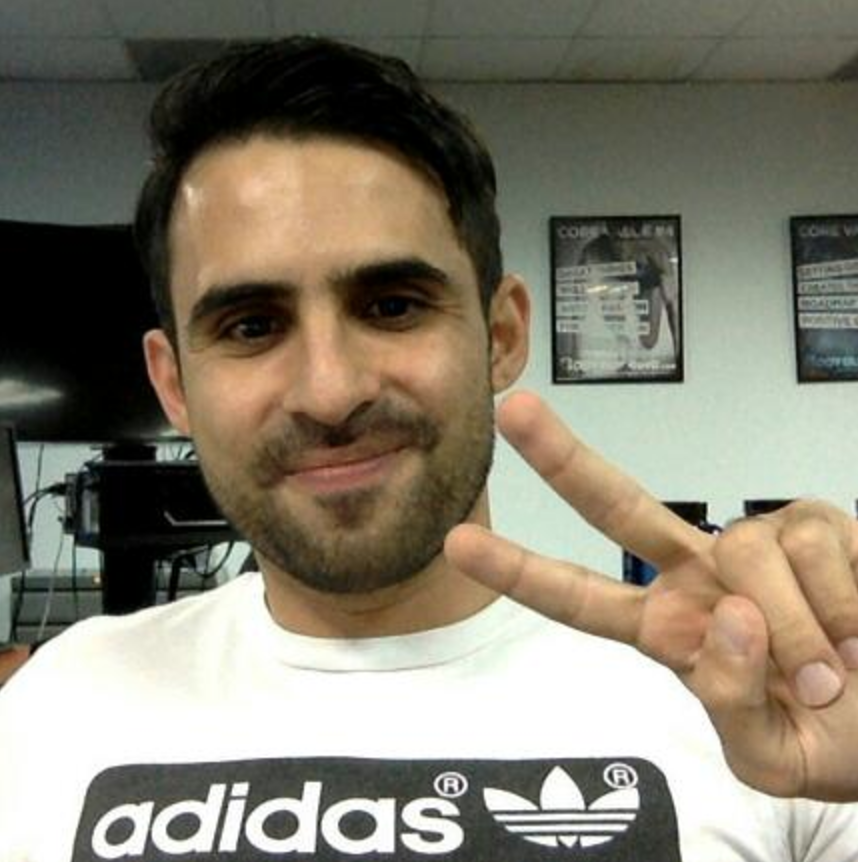
\includegraphics[width=1in,height=1.25in,clip,keepaspectratio]{martin-flores}}]{Martín Flores}
es Ingeniero en Informática de la Universidad Nacional. Actualmente, realiza sus estudios de Maestría en Ciencias de la Computación del Tecnológico de Costa Rica. Sus principales intereses son: lenguajes de programación, ingeniería de software y \emph{DevOps}.
\end{IEEEbiography}


% You can push biographies down or up by placing
% a \vfill before or after them. The appropriate
% use of \vfill depends on what kind of text is
% on the last page and whether or not the columns
% are being equalized.

%\vfill

% Can be used to pull up biographies so that the bottom of the last one
% is flush with the other column.
%\enlargethispage{-5in}



% that's all folks
\end{document}


